\documentclass[../../General.tex]{subfiles}
\begin{document}


\section{Concepto de solución óptimo}

Tras someter las alternativas de diseño a la evaluación técnica y económica, se declara a la solución 2 como el concepto de solución óptimo (ver Figura \ref{fig:EvalTecEc}). Al proyectar los puntajes en el gráfico de evaluación técnico-económica, esta alternativa presenta el mejor nivel de convergencia hacia la diagonal ideal, ofreciendo un excelenete desempeño industrial técnico sin incurrir en los costos excesivos.

\begin{figure}[H]
	\captionsetup{justification=raggedright, singlelinecheck=false, labelsep=none}
	
	\caption[Elaboración técnica económica de las tres soluciones propuestas.]{} 
	
	\textit{Elaboración técnica económica de las tres soluciones propuestas.} \par\medskip
	
	\centering
	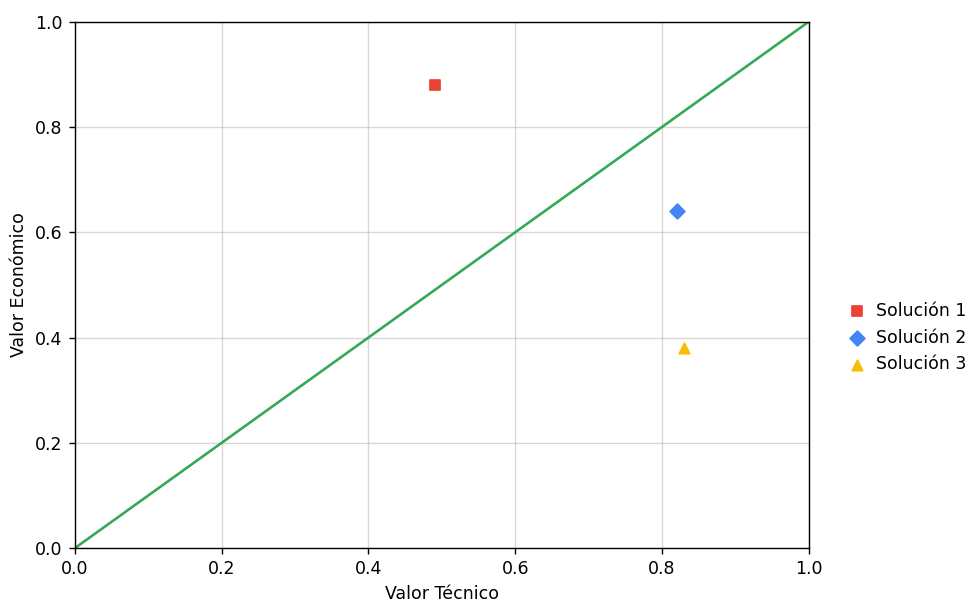
\includegraphics[width=0.8\textwidth]{Recursos/Imagenes/ImagenesConceptos/evtecec.png} \par\medskip
	
	\raggedright
	\footnotesize \textit{Nota.} Elaboración propia.
	\label{fig:EvalTecEc}
\end{figure}

% [COMPLETAR]: ALGUNAS COSAS QUE FALTAN EN ESTA SECCIÓN, SE DEBE DEFINIR MEJOR EL CONCEPTO DE SOLUCIÓN ÓPTIMO, REVISA OTRAS TESIS PARA VER QUÉ PONER AQUÍ.

\end{document}